\chapter{النسبية الخاصة: الأطر المرجعية، والتزامن، وتحويل لورنتز}

النسبية هي المبدأ القائل إن قوانين الفيزياء لا تعتمد على أي إطار قصوري نستخدمه لوصفها. ومهمتنا الأولى هي الحركيات: معنى المكان والزمان والحركة والمزامنة، والتحويل من إطار قصوري إلى آخر. أما الديناميكا فتأتي بعد ذلك، مع الطاقة النسبية، والزخم، والقوة، والنظير لمعادلة نيوتن للحركة، ومعنى \(E=mc^2\). وبمجرد أن يترسخ هذا البناء، يمكننا أن نقترب من النسبية العامة من الناحية المفاهيمية عبر الزمكان المنحني، وحركة الجسيمات في مجال ثقالي محدد سلفًا، والثقوب السوداء، وتمدد الكون، من غير أن نبدأ بالمشكلة الصعبة المتمثلة في حل معادلات حقل أينشتاين.

يجدر بنا أن نميز بين الصرامة المفاهيمية والصرامة الرياضية. لن نستخدم تقريبًا نعلم سلفًا أنه خاطئ. بل سنؤكد ما يفعله المجال الثقالي بالساعات والجسيمات والهندسة، مع إرجاء الأدوات اللازمة لبناء حلول اعتباطية لمعادلات الحقل. ويجب تناول النسبية الخاصة بمزيد من التصريح، لأن كل ذلك الاستدلال اللاحق يرتكز على حركياتها.

ولذلك فالموضع الصحيح للبدء ليس بمعادلة ذائعة الصيت، بل بعرض دقيق لما يعنيه الراصد بمكان وزمان.

\section{الإطار هو نظام إحداثيات فيزيائي}

تخيّل الفضاء مملوءًا بشبكة من مساطر مترية يمكن جعلها دقيقة بقدر ما نشاء. وتُعطى كل نقطة في الشبكة ثلاثة إحداثيات مكانية، وعند كل نقطة ساعة. وتكوّن القضبان والساعات معًا إطارًا مرجعيًا.

\begin{definition}
ال\emph{حدث} هو شيء يقع في مكان واحد وزمان واحد. في بُعد مكاني واحد تُكتب إحداثياته \((x,t)\)؛ وفي ثلاثة أبعاد تكون \((x,y,z,t)\).
\end{definition}

تضيف الفيزياء النيوتنية افتراضًا قويًا: يمكن مزامنة جميع الساعات المثالية مرة واحدة وإلى الأبد. الزمن كوني. قد تُنقل ساعة، وقد يحمل الراصد ساعة يد، لكن من المفترض أن يتفق الجميع على القيمة نفسها لـ \(t\) في كل مكان. ويُسمى هذا أحيانًا الزمن المطلق؛ ويمكن تصوره على أنه زمن الله، ساعة واحدة للعالم كله.

مبدأ النسبية أقدم من أينشتاين. وصورته الطبيعية هي قطار يتحرك بانتظام شديد فوق قضبان ملساء تمامًا بحيث لا شيء يقرع أو يهتز. وداخل القطار يمكننا أن نقذف الكرات ونلتقطها تمامًا كما نفعل في قطار واقف عند المحطة. إن التلاعب بالكرات تجربة صغيرة في الميكانيكا مكتملة على نحو يبعث على الدهشة: فهي تتطلب التوقيت، والجاذبية، والمحاذاة، والتحكم المتكرر في المسارات. وإذا كان القطار يتحرك بسرعة ثابتة، فلا تتغير أي من تلك القواعد. فالكرة المقذوفة مباشرة إلى أعلى تعود إلى اليد نفسها؛ ولا ينزلق القطار مبتعدًا من تحتها. وقد أدرك غاليليو هذه الحقيقة، وصاغها نيوتن على نحو منهجي في قوانين الحركة.

قبل غاليليو، كان من المغري أن نستدل بأن القطار المتحرك ينبغي أن يتقدم بينما تكون الكرة في الهواء، مما يضطر اللاعب إلى أن يمد يده إلى الخلف أو إلى الأمام ليستعيدها. والخطأ هو نسيان أن الكرة تشارك القطار بالفعل سرعته الأفقية حين تغادر اليد. ولا تكشف أي تجربة محصورة داخل العربة المتحركة بسلاسة عن حالة مميزة من السكون المطلق. إنما الحركة النسبية بين القطارين وحدها هي القابلة للرصد.

وعليه، فالقطار الساكن والقطار المتحرك حركة منتظمة هما إطاران قصوريان. وقبل أينشتاين، كانت العلاقة بينهما تُعطى بتحويلات غاليليو.

\section{رسم الزمكان}

نهمل \(y\) و\(z\) في الوقت الحاضر، ونرسم الزمن رأسيًا والموضع \(x\) أفقيًا. كل نقطة في الرسم تمثل حدثًا. والخط \(x=0\) هو تاريخ أصل المكان، أو \emph{خط العالم} الخاص به. أما الخطوط الرأسية المجاورة \(x=1,2,3,\ldots\) فهي خطوط العالم لنقاط الشبكة الأخرى. والخطوط الأفقية هي مجموعات من الأحداث ذات زمن مشترك.

\begin{figure}[H]
\centering
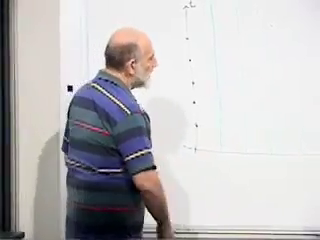
\includegraphics[width=0.62\textwidth]{lecture_01_figure_02.png}
\caption{محور الزمن في إطار السكون وأولى خطوط العالم للشبكة المكانية.}
\lectureframe{00:16:38}
\end{figure}

ويظهر البناء نفسه بوضوح أكبر في رسم مثالي:

\begin{figure}[H]
\centering
\begin{tikzpicture}[scale=0.95]
\draw[->] (-1.2,0) -- (5.2,0) node[right] {$x$};
\draw[->] (0,-0.2) -- (0,4.8) node[above] {$t$};
\foreach \x in {-1,1,2,3,4}
  \draw[gray!65] (\x,0) -- (\x,4.4);
\foreach \y in {1,2,3,4}
  \draw[gray!65] (-1.0,\y) -- (4.4,\y);
\fill (0,0) circle (1.5pt);
\node[below left] at (0,0) {$0$};
\node[left] at (0,1) {$1$};
\node[left] at (0,2) {$2$};
\node[left] at (0,3) {$3$};
\node[below] at (1,0) {$1$};
\node[below] at (2,0) {$2$};
\node[below] at (3,0) {$3$};
\end{tikzpicture}
\caption{شبكة زمكانية ساكنة. الخطوط الرأسية ذات موضع ثابت؛ والخطوط الأفقية ذات زمن ثابت.}
\end{figure}

هذه الشبكة تخيلية، وتباعدها اعتباطي. يمكننا أن نستخدم الأمتار، أو السنتيمترات، أو الميكرونات، أو أي فاصل أصغر من ذلك ما دام ذا معنى فيزيائي. وغرضها هو إسناد إحداثي دقيق إلى كل حدث.

إن عبارة «الإطار المرجعي» لها الآن معنى تشغيلي. فهي ليست مجرد وجهة نظر أو شخص ينظر في اتجاه ما. إنها جهاز إحداثيات ممتد. فإذا أُعطي حدث، حدّدت القضبان المحلية أين وقع وحددت الساعة المحلية متى وقع. وعندئذ يمكن مقارنة كميات فيزيائية أخرى بين الأطر: موضع جسيم وسرعته، وطاقته، وربما درجة حرارة جسم، وفي نهاية المطاف زخمه وقوته. وأبسط مقارنة هي التي تتضمن \(x\) و\(t\)، لذا نبدأ من هناك.

الآن ضع شبكة ثانية على قطار يتحرك في اتجاه \(x\) الموجب بسرعة ثابتة \(v\). واجعل الأصلين منطبقين عند \(t=0\). وعندئذ يتبع الأصل المتحرك
\begin{equation}
x=vt.
\end{equation}
وكل نقطة أخرى مثبتة في القطار تتبع خط عالم مائلاً موازيًا. وهذا الميل ليس إلا التعبير الهندسي عن أن القطار يغيّر موضعه مع مرور الزمن.

افترض أن النقطة الخلفية للقطار هي الأصل المعلَّم بشرطة. فعند \(t=0\) تنطبق على أصل المحطة. وعند زمن لاحق \(t\)، يكون إحداثيها في الإطار الساكن هو \(vt\). ولذلك يكون حدث قريب ذو الإحداثي \(x\) على بعد \(x-vt\) فقط من أصل القطار. ولهذا يكون التحويل طرحًا لا قاعدة جبرية اعتباطية.

ولتكن \((x,t)\) إحداثيات حدث في إطار المحطة، ولتكن \((x',t')\) إحداثياته في إطار القطار. يحتفظ غاليليو ونيوتن بزمن كوني،
\begin{equation}
t'=t.
\end{equation}
وخلال الزمن \(t\)، يتقدم الأصل المتحرك بمقدار \(vt\)، لذا تكون المسافة من ذلك الأصل إلى الحدث
\begin{equation}
x'=x-vt.
\end{equation}
ومعًا،
\begin{align}
t'&=t, & x'&=x-vt.
\label{eq:galilean-forward}
\end{align}
وبحل هذه العلاقات بالنسبة إلى الإحداثيات غير المعلَّمة بشرطة نحصل على التحويل العكسي،
\begin{align}
t&=t', & x&=x'+vt'.
\label{eq:galilean-inverse}
\end{align}

\begin{figure}[H]
\centering
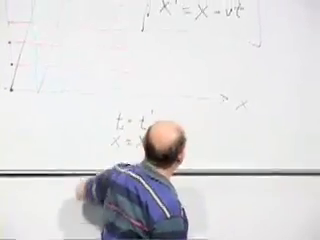
\includegraphics[width=0.72\textwidth]{lecture_01_figure_03.png}
\caption{تحويل غاليليو مكتوب بجانب شبكتي الزمكان.}
\lectureframe{00:21:57}
\end{figure}

يبين الزوج الأول للراصد المتحرك كيف يحوّل الإحداثيات التي يزوّده بها الراصد الساكن. والزوج العكسي يعيد التحويل. وهذا التحويل المتبادل بين الوصفين هو المضمون الرياضي لنسبية غاليليو.

إن الاستبدال \(t\to t'\) في الصيغة المكانية العكسية غير ضار إلا لأن نظرية غاليليو قد أعلنت بالفعل \(t=t'\). ومن المفيد أن نلحظ هذا الافتراض الآن. ففي نظرية أينشتاين سيختلف إحداثيا الزمن، ولن تعود مثل هذه الاستبدالات تلقائية.

\begin{classroomqa}
\audiencequestion{إذا حُمِلت ساعة بعيدًا ثم أُعيدت، فكيف يمكننا أن نعرف أن حركتها لم تُسرّعها أولًا ثم تُبطئها بعد ذلك، بحيث تُخفي الأثر عند مقارنة الساعات؟
\lecturetimestamp{00:23:09}}
\lecturerresponse{لم يكن في وسع غاليليو أن يثبت الزمن الكوني بدقة حديثة؛ فقد كان ذلك تخمينًا فيزيائيًا. ويمكننا اختبار هذا التخمين بطرائق كثيرة: نحمل ساعات جيدة في اتجاهين متعاكسين، ونكرر الرحلة شمالًا--جنوبًا وكذلك شرقًا--غربًا، أو نحرك ساعة حول الأخرى، أو نتبادل إشارات التوقيت من غير أن نجمع الساعات معًا. وعند السرعات العادية تتفق جميع هذه الاختبارات إلى دقة عالية جدًا. لكن مع ساعات ذات دقة كافية أو سرعات كبيرة بما فيه الكفاية يظهر بالفعل اختلاف صغير. وهذا الإخفاق للزمن الكوني ليس عيبًا في التجربة؛ بل هو إحدى الظواهر التي يجب على النسبية الخاصة أن تفسرها.}
\end{classroomqa}

\section{الثوابت الغاليليّة وقانون نيوتن}

الثابت هو كمية يتفق عليها جميع الراصدين القصوريين المعنيين هنا. وليس من الضروري أن تكون الإحداثيات نفسها ثابتة. وما يهم هو ما إذا كانت القوانين المؤلَّفة منها تحتفظ بالشكل نفسه.

تُستعمل هذه الكلمة اسمًا وصفةً معًا. فيمكن أن يكون عدد ما ثابتًا، ويمكن أن تكون معادلة ثابتةً تحت تحويل ما. والتمييز بين الكميات الثابتة والقوانين الثابتة يمنع التباسًا شائعًا: فالنسبية لا تدّعي أن كل راصد يعيّن لكل شيء الإحداثي نفسه. بل تدّعي أن القانون الفيزيائي الذي يربط قياساتهم له الشكل نفسه.

اعتبر حدثين متزامنين عند الموضعين \(x_1\) و\(x_2\). تعطي المعادلة~\eqref{eq:galilean-forward}
\begin{align}
x_1'&=x_1-vt,\\
x_2'&=x_2-vt.
\end{align}
ومن ثم فإن المسافة بينهما هي
\begin{equation}
x_2'-x_1'=(x_2-vt)-(x_1-vt)=x_2-x_1.
\end{equation}
في فيزياء غاليليو، تكون المسافة بين حدثين يقعان في الوقت نفسه ثابتة، رغم أن الموضعين المفردين ليسا كذلك.

\begin{classroomqa}
\audiencequestion{هل موضعا \(t\) في ذلك الطرح هما فعلًا الزمن نفسه؟
\lecturetimestamp{00:28:16}}
\lecturerresponse{نعم. لقد اخترنا الحدثين عمدًا ليكونا \((x_1,t)\) و\((x_2,t)\). وهما يقعان على خط أفقي واحد لزمن ثابت. ولذا فإن الحد المشترك \(vt\) يُلغى. ولو وقعت الأحداث عند أزمنة مختلفة، لما كانت هذه الحجة لتثبت فاصلًا مكانيًا لا يتغير.}
\end{classroomqa}

لنصف الآن جسيمًا بمسار \(x(t)\). ويعطي راصد القطار
\begin{equation}
x'(t)=x(t)-vt.
\end{equation}
وبأخذ المشتقة مرة واحدة نحصل على قاعدة جمع السرعات المألوفة،
\begin{equation}
\frac{dx'}{dt}=\frac{dx}{dt}-v.
\end{equation}
فالموضع والسرعة يعتمدان على الإطار المرجعي. فالراصد الذي يتحرك بمحاذاة سهم يراه يتحرك أبطأ من راصد يقف إلى جانب السكة.

خذ المشتقة مرةً أخرى. وبما أن السرعة النسبية \(v\) ثابتة،
\begin{equation}
\frac{d^2x'}{dt^2}=\frac{d^2x}{dt^2}.
\end{equation}
فالتسارع لا يتغير تحت تحويل غاليلي. وهذا يوحي بقوة بسبب كتابة قانون نيوتن بدلالة التسارع لا بدلالة الموضع أو السرعة.

هذا هو تسارع الجسم المرصود، لا تسارع راصد القطار. فكلا الإطارين عطالي، ولذلك لا يتسارع أيٌّ منهما بالنسبة إلى الآخر. وقد تتسارع الأجسام إلى اليسار أو إلى اليمين في أيٍّ من الوصفين، ويتفق الراصدان على قيمة ذلك التسارع مع أنهما يختلفان في موضع الجسم وسرعته.

افترض أن جسيمين يؤثر كلٌّ منهما في الآخر بقوة، وأن هذه القوة لا تعتمد إلا على المسافة الفاصلة بينهما عند اللحظة نفسها. هذه المسافة لا تتغير، ولذلك لا تتغير القوة. وإذا كانت الكتلة أيضًا خاصية جوهرية لا تعتمد على الإطار، فإن كل راصد عطالي يستطيع أن يكتب
\begin{equation}
F=ma
\end{equation}
بالصيغة نفسها تمامًا. فالميكانيكا النيوتنية لا تتغير تحت التحويلات الغاليلية. وليس هذا مجرد أمر معقول؛ بل هو بالغ الدقة على نحو استثنائي في مجال السرعات المألوفة كله.

تنطبق الحجة على القوى المركزية المألوفة مثل الجاذبية النيوتنية أو الكهروستاتيكا، حيث يكون المقدار دالة في المسافة. وبما أن جميع الراصدين في الأطر الغاليلية يتفقون على تلك المسافة عند زمن مشترك، فإنهم يتفقون على القوة. ومع ثبات القوة والتسارع، يقتضي الاتساق عندئذ أن يتفقوا على الكتلة أيضًا: فالجسم ذو الكيلوغرام الواحد يبقى جسمًا ذا كيلوغرام واحد عندما يمر محمولًا في قطار. وكل رمز في \(F=ma\) ينسجم مع البنية نفسها التي لا تتغير.

\section{الضوء لا ينسجم مع القاعدة الغاليلية}

الكهرومغناطيسية هي التي تولِّد هذه الصعوبة. فمعادلات ماكسويل تتنبأ بموجات تنتقل عبر الفضاء الخالي بسرعة محددة \(c\). فإذا كانت معادلات ماكسويل من قوانين الطبيعة، وكانت قوانين الطبيعة هي نفسها في كل إطار عطالي، وجب على جميع الراصدين العطاليين أن يحصلوا على القيمة نفسها \(c\).

لكن الحركيات الغاليلية تتنبأ بشيء آخر. فنبضة ضوئية تتحرك نحو اليمين في الإطار الساكن تحقق
\begin{equation}
x=ct.
\end{equation}
وبتطبيق التحويل المكاني نحصل على
\begin{equation}
x'=x-vt=(c-v)t.
\end{equation}
وبما أن \(t'=t\)، فإن راصد القطار سيقيس السرعة \(c-v\).

يمكن صياغة التناقض على نحو حاسم. فإذا احتفظت معادلات ماكسويل بصيغتها، فإنها تتنبأ بـ \(c\) في الإطار المشار إليه بشرطة. وإذا أُبقي على التحويل الغاليلي، فإنه يتنبأ بـ \(c-v\). ولا يمكن أن يكون كلاهما دقيقًا تمامًا عندما يكون \(v\ne0\).

تبدو هذه النتيجة طبيعية تمامًا إذا كان الضوء يتصرف كموجة عادية في وسط. فالقارب الذي يتحرك مع موجة مائية يقيس سرعة موجية نسبية أقل. والمستمع الذي يتحرك خلال هواء ساكن يقيس سرعةً للصوت تنزاح بسبب حركة المستمع بالنسبة إلى الهواء. ولذلك انجذب فيزيائيو القرن التاسع عشر إلى فكرة حالة سكون مفضلة، أي إطار أثيري تكون فيه معادلات ماكسويل في أبسط صورة لها ويتحرك فيه الضوء بسرعة \(c\). غير أن التجارب المصممة لكشف الحركة بالنسبة إلى مثل هذا الإطار المفضل لم تجد أثرًا مطابقًا لذلك.

كانت هناك ترتيبات تجريبية ممكنة عدة، لكن هدفها المشترك كان مقارنة انتشار الضوء لدى راصدين في حالات حركة مختلفة أو اتجاهات مختلفة للحركة. ولم يكشف أيٌّ منها عن الانزياح الغاليلي المتوقع. ولم يكن هذا الإخفاق مجرد إزعاج تقني صغير. بل فرض الاختيار بين مبدأ النسبية، ومعادلات ماكسويل، والتصورات الموروثة عن المكان والزمان.

تناول أينشتاين هذا التعارض على نحو أكثر مباشرة. فقد تخيل في شبابه أنه يطارد موجة ضوئية. ولو استطاع اللحاق بها، لتجمَّد نمطها الكهرومغناطيسي المتذبذب في الفضاء، مع أن معادلات ماكسويل لا تسمح بمثل هذه الموجة الضوئية الساكنة. فاختار أن يعدّ نظرية ماكسويل ومبدأ النسبية أمرين أساسيين، ثم يعيد النظر في الافتراضات الكامنة في إحداثياتنا.

تقوم إعادة البناء على مسلَّمتين:
\begin{enumerate}
\item تأخذ قوانين الفيزياء الصيغة نفسها في كل إطار عطالي.
\item للضوء في الفراغ السرعة نفسها \(c\) في كل إطار عطالي.
\end{enumerate}

لا يمكن للمسلَّمة الثانية أن تتعايش مع التحويل الغاليلي. فلا بد أن يتغير شيء أعمق من قاعدة جمع السرعات. وكان خيار أينشتاين الأكثر اقتصادًا هو الإبقاء على المسلَّمتين وإعادة النظر في المعادلة الغاليلية البريئة في ظاهرها \(t'=t\).

\section{مزامنة الساعات البعيدة}

يمكن تعيين المسافات المكانية بقضبان القياس، لكن الساعات البعيدة تتطلب اصطلاحًا للمزامنة. ضع ساعتين على مسافتين متساويتين من راصد في المنتصف. وعندما تقرأ كل ساعة عند الطرف الوقت المعيَّن، فلتطلق ومضة. فإذا وصلت الومضتان إلى المنتصف معًا، فاعتبر ساعتي الطرف متزامنتين. وإذا وصلت إحدى الومضتين أولًا، فاضبط الساعة المناظرة وكرر الإجراء.

وتُعرَّف كلمة \emph{المنتصف} باستخدام قضبان القياس التي سبق وضعها في ذلك الإطار. ولذلك يتضمن الاختبار عنصرين منفصلين: تساوي المسافة المكانية عن الطرفين، وتساوي زمن وصول الإشارتين. ولا يجوز إسقاط أيٍّ من هذين العنصرين. وتكرار الإجراء في أنحاء الشبكة كلها يزوِّدنا بالخطوط الأفقية ذات الزمن الثابت التي كان نيوتن قد افترضها ببساطة.

ويستخدم هذا التعريف الضوء لأن المسلَّمة تعطي الضوء السرعة نفسها في كل إطار عطالي. وما إن تُعالَج جميع الأزواج المتجاورة بهذه الطريقة حتى تحمل الشبكة كلها مجموعة متزامنة من الساعات.

ولندع الآن شبكةً ثانية تتحرك خلال الأولى. فمنتصف الجهاز المتحرك يبقى في منتصف المسافة بين طرفيه المتحركين في إطاره الخاص. أما بالنسبة إلى الجهاز الساكن، فإنه يتحرك نحو إحدى الومضتين القادمتين ويبتعد عن الأخرى. والومضتان المنبعثتان في آن واحد وفقًا للساعات الساكنة لا تصلان معًا إلى المنتصف المتحرك. وبما أن الراصد المتحرك يطبق قاعدة المنتصف والضوء نفسها، فلا يستطيع أن يعدَّ هذين الانبعاثين متزامنين. فكل إطار يزامن ساعاته الخاصة على نحو متسق، لكن عمليتي المزامنة لا تتفقان.

وهذا ليس خداعًا بصريًا ناتجًا عن محدودية زمن انتقال الضوء. فكل راصد يعلم أن الضوء يستغرق وقتًا ليصل، ويصحح أثر ذلك باستخدام السرعة نفسها \(c\). ويظل الخلاف قائمًا بعد هذا التصحيح لأن الراصدين لا يختاران الحدثين البعيدين نفسيهما على أنهما زوج متزامن. فالتزامن نفسه، لا مجرد مظهر التزامن، نسبي.

\begin{classroomqa}
\audiencequestion{هل يمكننا تجنب هذا الاستنتاج بمزامنة الساعات بالصوت بدلًا من الضوء؟
\lecturetimestamp{00:49:03}}
\lecturerresponse{يصلح الصوت إشارةً للمزامنة في إطار يكون فيه الهواء ساكنًا، لكن سرعته المقاسة ليست هي نفسها في كل إطار عطالي. فالقطار المفتوح الذي يتحرك خلال هواء ساكن يكون متحركًا بالنسبة إلى الوسط الحامل للصوت، ولذلك لا تتصرف إشارات الصوت المتجهة إلى الأمام وإلى الخلف فيه على نحو متناظر. أما الضوء فمختلف بحسب المسلَّمة: لا يوجد وسط بصري قابل للكشف يحدد إطار سكونه راصدًا بعينه. ولذلك نستخدم الضوء ونتبع النتائج المترتبة على ذلك.}
\end{classroomqa}

أصبح الخلاف النوعي واضحًا. ونحسب الآن على وجه الدقة أيَّ الأحداث يعدها الراصد المتحرك متزامنة.

\section{بناء أشعة الضوء}

ولأجل هذا البناء، من الملائم اختيار وحدات بحيث
\begin{equation}
c=1.
\end{equation}
وعندئذ تكون وحدة المسافة هي المسافة التي يقطعها الضوء في وحدة واحدة من الزمن: ثوانٍ ضوئية مقترنة بثوانٍ، أو سنوات ضوئية مقترنة بسنوات. ويُقاس المكان والزمان بالوحدات نفسها، وتكون السرعات بلا أبعاد، وتظهر أشعة الضوء عند \(45^\circ\). فالشعاع المتحرك نحو اليمين يحقق
\begin{equation}
x=t+d,
\end{equation}
بينما يحقق الشعاع المتحرك نحو اليسار
\begin{equation}
x=-t+d'.
\end{equation}
وأما الشعاعان الماران بنقطة الأصل فهما ببساطة \(x=t\) و\(x=-t\). وتقع المسارات الزمنية، التي تخص أجسامًا أبطأ من الضوء، أقرب إلى المحور الرأسي. أما مسار افتراضي أسرع من الضوء فسيقع أقرب إلى المحور الأفقي.

لا تصبح الزاوية في الرسم ذات معنى إلا بعد اختيار هذه الوحدات. فبوحدتي المتر والثانية سيبدو الشعاع الضوئي أفقيًا تقريبًا لأنه يقطع نحو \(3\times10^8\) متر في ثانية واحدة. واختيار الثواني الضوئية للمسافة يعيد تحجيم المحور الأفقي ويجعل الهندسة السببية مرئية.

اعتبر ثلاثة خطوط عالم متوازية في الشبكة المتحركة،
\begin{equation}
x=vt,\qquad x=vt+L,\qquad x=vt+2L.
\label{eq:moving-worldlines}
\end{equation}
ينتمي خط العالم الأوسط إلى الراصد الذي يختبر التزامن بين النقطتين الطرفيتين. تتحرك النقاط الثلاث بانتظام وتحافظ على ترتيبها النسبي في الإطار ذي الشرطة.

\begin{figure}[H]
\centering
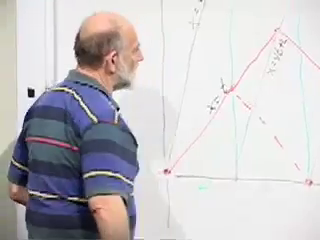
\includegraphics[width=0.72\textwidth]{lecture_01_figure_04.png}
\caption{الشعاع الضوئي المتجه إلى الأمام \(x=t\) عند التقائه بخط العالم المتحرك الأوسط.}
\lectureframe{01:02:33}
\end{figure}

يمكن رسم الهندسة الكاملة من دون أن يحجبها شخص واقف أمام اللوح:

\begin{figure}[H]
\centering
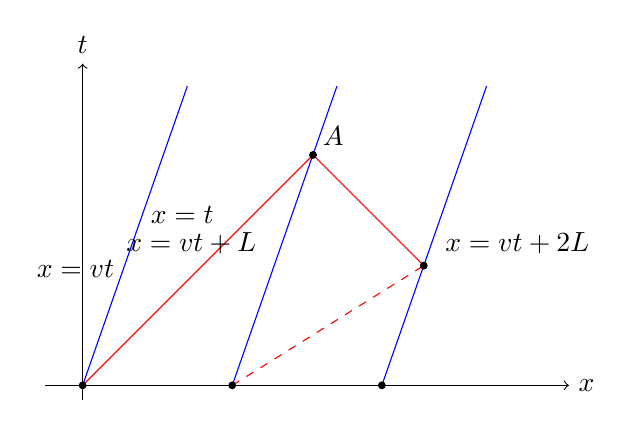
\begin{tikzpicture}[scale=0.95]
\draw[->] (-0.5,0) -- (6.5,0) node[right] {$x$};
\draw[->] (0,-0.2) -- (0,4.3) node[above] {$t$};
\draw[blue] (0,0) -- (1.4,4.0);
\draw[blue] (2.0,0) -- (3.4,4.0);
\draw[blue] (4.0,0) -- (5.4,4.0);
\draw[red] (0,0) -- (3.08,3.08);
\draw[red] (3.08,3.08) -- (4.56,1.60);
\draw[red,dashed] (2.0,0) -- (4.56,1.60);
\fill (0,0) circle (1.5pt);
\fill (2.0,0) circle (1.5pt);
\fill (4.0,0) circle (1.5pt);
\fill (3.08,3.08) circle (1.5pt);
\fill (4.56,1.60) circle (1.5pt);
\node[left] at (0.55,1.55) {$x=vt$};
\node[left] at (2.45,1.9) {$x=vt+L$};
\node[right] at (4.72,1.9) {$x=vt+2L$};
\node[left] at (1.88,2.28) {$x=t$};
\node[above right] at (3.08,3.08) {$A$};
\end{tikzpicture}
\caption{تحدد الإشارات الضوئية خط التزامن في الإطار المتحرك.}
\end{figure}

أرسل شعاعًا ضوئيًا متجهًا إلى اليمين من الأصل. لتكن \(A\) نقطة تقاطعه مع خط العالم الأوسط. والمعادلتان عند \(A\) هما
\begin{align}
x&=t,\\
x&=vt+L.
\end{align}
وبالتعويض نحصل على
\begin{equation}
t=vt+L,
\end{equation}
ومن ثم
\begin{equation}
t_A=x_A=\frac{L}{1-v}.
\label{eq:point-a}
\end{equation}

ابتداءً من \(A\)، تتبَّع شعاعًا ضوئيًا متجهًا إلى اليسار رجوعًا حتى خط العالم المتحرك الأيمن. معادلته تأخذ الصورة
\begin{equation}
x+t=b.
\end{equation}
ولأنه يمر عبر \(A\)، فإن المعادلة~\eqref{eq:point-a} تحدد الثابت:
\begin{equation}
b=x_A+t_A=\frac{2L}{1-v}.
\end{equation}
ولذلك يحقق الشعاع الراجع
\begin{equation}
x+t=\frac{2L}{1-v}.
\label{eq:backward-ray}
\end{equation}

ويُستنتَج تقاطعه مع خط العالم الأيمن من
\begin{align}
x+t&=\frac{2L}{1-v},\\
x&=vt+2L.
\end{align}
وبحذف \(x\)،
\begin{align}
(1+v)t
  &=2L\left(\frac{1}{1-v}-1\right)\\
  &=\frac{2Lv}{1-v},
\end{align}
إذن
\begin{equation}
t=\frac{2Lv}{1-v^2}.
\end{equation}
وبالتعويض في \(x=vt+2L\) نحصل على
\begin{equation}
x=\frac{2L}{1-v^2}.
\end{equation}
الإحداثيات نفسها أقل أهمية من نسبتها:
\begin{equation}
\frac{t}{x}=v.
\end{equation}
ومن ثم فإن كل حدث متزامن مع الأصل وفقًا للساعات المتحركة يقع على
\begin{equation}
t=vx,
\label{eq:simultaneity-c-one}
\end{equation}
بينما يتبع أصل الإطار المتحرك
\begin{equation}
x=vt.
\label{eq:moving-time-axis}
\end{equation}
والمحوران مائلان تناظريًا حول شعاع الضوء عند \(45^\circ\).

كل النقاط على \(x=vt\) لها الموضع ذو الشرطة نفسه، \(x'=0\)، بينما تختلف أزمنتها ذات الشرطة. وكل النقاط على \(t=vx\) لها الزمن ذو الشرطة نفسه، \(t'=0\)، بينما تختلف مواضعها ذات الشرطة. ولذلك فإن الأول هو محور الزمن ذي الشرطة والآخر محور المكان ذي الشرطة. وكان بناء الإشارات الطويل ضروريًا لتعيين الخط الثاني؛ إذ لم يكن من الممكن استنتاجه من خط العالم المتحرك وحده.

إن إرجاع الوحدات المعتادة في المعادلة~\eqref{eq:simultaneity-c-one} يتطلب
\begin{equation}
t=\frac{v}{c^2}x.
\label{eq:simultaneity-dimensional}
\end{equation}
ويفسر العامل \(c^2\) لماذا تعمل الصورة النيوتنية جيدًا إلى هذا الحد في الحياة اليومية. فعند السرعات الصغيرة جدًا مقارنةً بـ \(c\)، يكون ميل خط التزامن المتحرك صغيرًا للغاية.

\begin{figure}[H]
\centering
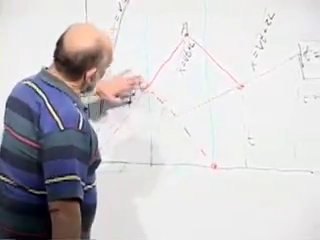
\includegraphics[width=0.72\textwidth]{lecture_01_figure_05.png}
\caption{مع \(c=1\)، يكون محورا الزمن ذي الشرطة والتزامن متماثلين حول شعاع الضوء.}
\lectureframe{01:15:40}
\end{figure}

\begin{figure}[H]
\centering
\begin{tikzpicture}[scale=1.0]
\draw[->] (-2.2,0) -- (5.2,0) node[right] {$x$};
\draw[->] (0,-0.2) -- (0,4.9) node[above] {$t$};
\draw[red] (0,0) -- (3.9,3.9);
\draw[red] (0,0) -- (-1.8,1.8);
\draw[blue] (0,0) -- (1.8,4.5);
\draw[blue,dashed] (0,0) -- (4.5,1.8);
\node[right] at (3.9,3.9) {$x=t$};
\node[left] at (-1.8,1.8) {$x=-t$};
\node[above] at (1.8,4.5) {$x'=0$};
\node[right] at (4.5,1.8) {$t'=0$};
\end{tikzpicture}
\caption{المحاور ذات الشرطة وأشعة الضوء الثابتة في وحدات \(c=1\).}
\end{figure}

\section{اشتقاق تحويل لورنتز}

تحدد الهندسة المواضع التي تنعدم عندها كل إحداثية ذات شرطة. فعلى امتداد محور الزمن المتحرك \(x=vt\)، يجب أن يكون \(x'=0\). وعلى امتداد محور التزامن المتحرك \(t=vx\)، يجب أن يكون \(t'=0\). ويمكن كتابة أعم العلاقات الخطية الموافقة لمواضع الانعدام هذه على الصورة
\begin{align}
x'&=\frac{x-vt}{F(v)},\\
t'&=\frac{t-vx}{G(v)}.
\label{eq:fg-ansatz}
\end{align}
ويسمح العاملان \(F\) و\(G\) بأن تختلف مقاييس الإحداثيات ذات الشرطة عن المقاييس الغاليلية، مع أن موضعي المحورين قد تحددا بالفعل. وتنتج الخطية من تجانس المكان والزمان: فنقل تجربة من موضع إلى آخر لا يمكن أن يغيّر قانون التحويل.\editorialnote{هذه الحجة الموجزة للخطية تُصرِّح بافتراض استُخدم ضمنًا في الاشتقاق على اللوح.}

في هذه المرحلة أخبرتنا الهندسة بالكثير، ولكن ليس بكل شيء. فالبسطان يحددان ميل المحورين، لكنهما لا يحددان تباعد الوحدات على امتدادهما. وهذه المعلومة المقياسية المتبقية هي بالضبط ما يمثله \(F(v)\) و\(G(v)\).

لنفرض الآن ثبات سرعة الضوء. فشعاع متجه إلى اليمين يحقق \(x=t\) يجب أن يحقق أيضًا \(x'=t'\). وعلى طول ذلك الشعاع،
\begin{align}
x'&=\frac{(1-v)t}{F(v)},\\
t'&=\frac{(1-v)t}{G(v)}.
\end{align}
ولكي تتحقق المساواة عند كل نقطة على الشعاع، لا بد من أن
\begin{equation}
F(v)=G(v).
\end{equation}
ولذلك يمكننا أن نكتب
\begin{align}
x'&=\frac{x-vt}{F(v)},\\
t'&=\frac{t-vx}{F(v)}.
\label{eq:common-f}
\end{align}

تستخدم هذه الخطوة أول مطلب أينشتايني حقيقي في الجبر. فالخط الهندسي نفسه هو شعاع ضوئي بالنسبة إلى كلا الراصدين، لذا يجب أن يزداد الإحداثيان ذوا الشرطة بالمقدار نفسه على امتداده عندما يكون \(c=1\). ولو اختلف العاملان في المعادلتين لكانت السرعة ذات الشرطة مختلفة عن الواحد.

يبقى تابع مجهول واحد. اضرب المعادلة~\eqref{eq:common-f} في \(F(v)\):
\begin{align}
F(v)x'&=x-vt,\\
F(v)t'&=t-vx.
\end{align}
وبضرب المعادلة الثانية في \(v\) ثم جمعها مع الأولى يُحذَف \(t\)، فنحصل على
\begin{equation}
(1-v^2)x=F(v)(x'+vt').
\end{equation}
وبالمثل،
\begin{equation}
(1-v^2)t=F(v)(t'+vx').
\end{equation}
ولذلك يكون التحويل العكسي
\begin{align}
x&=\frac{F(v)}{1-v^2}(x'+vt'),\\
t&=\frac{F(v)}{1-v^2}(t'+vx').
\end{align}

يجعل مبدأ النسبية العلاقة بين الإطارين تبادلية. فإذا رأت المحطة القطار يتحرك بسرعة \(+v\)، فإن القطار يرى المحطة تتحرك بسرعة \(-v\). وبناءً على ذلك، يجب أن تكون المعادلات العكسية على الصورة نفسها التي للمعادلات الأمامية مع عكس إشارة \(v\). ويجب أن تحقق معاملاتها الأمامية
\begin{equation}
\frac{F(v)}{1-v^2}=\frac{1}{F(v)}.
\end{equation}
ومن ثم
\begin{equation}
F(v)^2=1-v^2,
\end{equation}
ويختار الاتصال مع تحويل الهوية عند \(v=0\) الجذر الموجب،
\begin{equation}
F(v)=\sqrt{1-v^2}.
\end{equation}

لم تُواءَم النتيجة مع نبضة ضوئية بعينها. فهي تنشأ من المحاور التي يثبتها التزامن، ومن السرعة المشتركة للضوء، ومن اشتراط ألا يُمنَح أي إطار قصوري امتيازًا على الآخر.

تحويل لورنتز بوحدات يكون فيها \(c=1\) هو
\begin{align}
x'&=\frac{x-vt}{\sqrt{1-v^2}},\\
t'&=\frac{t-vx}{\sqrt{1-v^2}}.
\label{eq:lorentz-c-one}
\end{align}
ومعكوسه هو
\begin{align}
x&=\frac{x'+vt'}{\sqrt{1-v^2}},\\
t&=\frac{t'+vx'}{\sqrt{1-v^2}}.
\end{align}

\begin{figure}[H]
\centering
\includegraphics[width=0.76\textwidth]{lecture_01_figure_06.png}
\caption{تحويل لورنتز المكتمل في وحدات \(c=1\) على اللوح.}
\lectureframe{01:32:38}
\end{figure}

تظهر الحداثة الأساسية بالفعل في معادلة الزمن. فالزمن لا يُنقل ببساطة من إطار إلى آخر من دون تغيّر. إذ يمزج إحداثي الزمن ذي الشرطة بين الزمن والموضع في الإطار غير المعلَّم بالشرطة. ونتيجةً لذلك، فإن \(t=\text{constant}\) و\(t'=\text{constant}\) يصفان مجموعتين مختلفتين من الأحداث.

حدّ المزج ليس تصحيحًا اختياريًا يُلحَق لاحقًا. فبدونه سيبقى الخط \(t'=0\) أفقيًا، وسيظل تزامن الأحداث البعيدة كونيًا، ولن يستطيع التحويل أن يحفظ سرعة الضوء.

\section{استعادة سرعة الضوء والتحقق من النتيجة}

عندما يكون \(c\ne1\)، يعيد الاتساق البعدي العوامل الناقصة. فالنسبة \(v^2/c^2\) لا بُعدية، بينما \((v/c^2)x\) له وحدات زمن. ومن ثم
\begin{align}
x'&=\frac{x-vt}{\sqrt{1-v^2/c^2}},\\
t'&=\frac{t-(v/c^2)x}{\sqrt{1-v^2/c^2}}.
\label{eq:lorentz-dimensional}
\end{align}
ويُحصَل على المعكوس بعكس إشارة \(v\):
\begin{align}
x&=\frac{x'+vt'}{\sqrt{1-v^2/c^2}},\\
t&=\frac{t'+(v/c^2)x'}{\sqrt{1-v^2/c^2}}.
\end{align}
ومن شأن إدخال
\begin{equation}
\gamma=\frac{1}{\sqrt{1-v^2/c^2}}
\end{equation}
أن يضع هذه المعادلات في الصيغة الموجزة المألوفة، لكن صيغة المقام تُبقي الاشتقاق ظاهرًا.

عدديًا، \(c\simeq3\times10^8\,\mathrm{m/s}\)، ومن ثم \(c^2\simeq9\times10^{16}\,\mathrm{m^2/s^2}\). ويجعل هذا المقام الكبير كلاً من ميل خط التزامن والعامل \(v^2/c^2\) غير ملحوظين في معظم التجارب الميكانيكية. وهذا الصغر يفسر نجاح غاليليو؛ لكنه لا يعيد الزمن المطلق.

\begin{figure}[H]
\centering
\includegraphics[width=0.76\textwidth]{lecture_01_figure_07.png}
\caption{تحويل لورنتز بعد استعادة عوامل \(c\).}
\lectureframe{01:35:58}
\end{figure}

هناك اختباران مباشران. خذ أولًا \(v\ll c\). عندئذٍ يكون \(v^2/c^2\) مهمَلًا، وللمسافات العادية يكون حد نسبية التزامن \(vx/c^2\) مهمَلًا أيضًا. وتختزل المعادلة~\eqref{eq:lorentz-dimensional} إلى
\begin{equation}
t'\approx t,\qquad x'\approx x-vt.
\end{equation}
وتُستعاد النسبية الغاليلية بوصفها تقريب السرعات المنخفضة.

ثانيًا، اختبر شعاعًا ضوئيًا. فبعد استعادة \(c\)، يحقق الشعاع المتجه إلى اليمين \(x=ct\)، لا \(x=t\). ويعطي التعويض
\begin{align}
x'&=\frac{(c-v)t}{\sqrt{1-v^2/c^2}},\\
t'&=\frac{(1-v/c)t}{\sqrt{1-v^2/c^2}}.
\end{align}
وبما أن \(c-v=c(1-v/c)\)،
\begin{equation}
x'=ct'.
\end{equation}
فإن الراصد في الإطار ذي الشرطة يقيس السرعة نفسها \(c\). وبالنسبة إلى شعاع متجه إلى اليسار، فإن التعويض عن \(x=-ct\) يعطي بالمثل
\begin{equation}
x'=-ct'.
\end{equation}
ويتعامل التحويل مع الضوء المتحرك في أي من الاتجاهين على نحو صحيح.

إن التمييز بين \(x=t\) و\(x=ct\) فحصٌ بُعديٌّ مفيد. فالأولى صحيحة فقط في وحدات يكون فيها \(c=1\). وإن استعادة الوحدات المعتادة في التحويل مع إبقاء معادلة الشعاع في الوحدات الطبيعية سيخلط بين اصطلاحين ويؤدي إلى نتيجة خاطئة. ويلتقط الاتساق البعدي هذا الخطأ فورًا.

\section{معيار نقطة المنتصف}

\begin{classroomqa}
\audiencequestion{افترض أن راصدًا يستقبل وميضين في اللحظة نفسها، لكنه ليس في منتصف المسافة بين مصدريهما. فهل يجوز لذلك الراصد أن يستنتج أن الوميضين قد انبعثا في آن واحد؟
\lecturetimestamp{01:42:55}}
\lecturerresponse{لا. إن تساوي زمنَي الوصول لا يستلزم تساوي زمنَي الانبعاث إلا بالنسبة إلى الراصد الواقع مكانيًا في منتصف المسافة بين المصدرين في الإطار المعني. فالمستقبِل الأقرب إلى أحد المصدرين قد يتلقى الوميضين معًا مع أن الوميض الأبعد قد انبعث أبكر. ولذلك فإن خط عالم المنتصف \(x=vt+L\) أساسي في البنية المتحركة. ويُتتبَّع الشعاع المتجه إلى الأمام \(x=t\) حتى يلتقي بخط المنتصف ذاك، ثم يُتتبَّع شعاع ضوئي راجع حتى \(x=vt+2L\). وذلك الحدث الطرفي الثاني، لا حدث وصول متساوٍ اعتباطي في موضع آخر، هو المتزامن مع الأصل وفقًا للإطار المتحرك.}
\end{classroomqa}

لقد بلغنا تحويل الإحداثيات الكامل، ولكننا لم نصل بعد إلى أشهر نتائجه. ويأتي بعد ذلك تقلص الطول وتمدد الزمن والزمن الخاص، ثم الزخم والطاقة النسبيان. والأساس قائم بالفعل: فلا يستطيع كل إطار قصوري أن يستخدم القوانين نفسها ويقيس سرعة الضوء نفسها إلا لأن المكان والزمان يمتزجان، ولأن تزامن الأحداث البعيدة ينتمي إلى إطار ما بدلًا من أن ينتمي إلى العالم على نحو مطلق.